\section{Contacting Graphene Nanoribbons}

The technique of connecting graphene nanoribbons is one of the greatest challenges to the development of reliable and robust electronics. Standard metal deposition processes can be used to contact lithographic ribbons by coating the substrate with a resist and evaporating metals. As described in Ch.~\ref{ch:introduction}, bulk graphene in contact with metals will produce finite Schottky barriers. Liquid-processable \glspl{GNR} offer a step forward in terms of structural integrity and edge shape. The placement of such structures on top of a device presents, however, one of the greatest obstacles to the use of ribbons in solutions. This scenario can be logically related to Buffon's needle problem, a well-known problem in geometric probability.

The Buffon's needle problem, first proposed in the eighteenth century, estimates the likelihood that by randomly tossing a needle of length $l$ this will touch at least one line of a group of parallel lines separated by a distance $d > l$. Even if no interactions between the needle and the grid are assumed, the problem captures the core of our experiment. The probability that the needle intersects at least one line can be computed analytically in the limit where $\lambda = l/d > 1$~\cite{uspensky1937introduction}

\begin{equation}
    P(\lambda) =
    \begin{cases}
        \frac{2\lambda}{\pi}                                                   & \lambda\leq 1 \\
        \frac{2}{\pi}\qty(\lambda - \sqrt{\lambda^2 - 1} + \sec^{-1}(\lambda)) & \lambda>1     \\
    \end{cases}
\end{equation}
%
\begin{figure}[hbtp]
    \begin{center}
        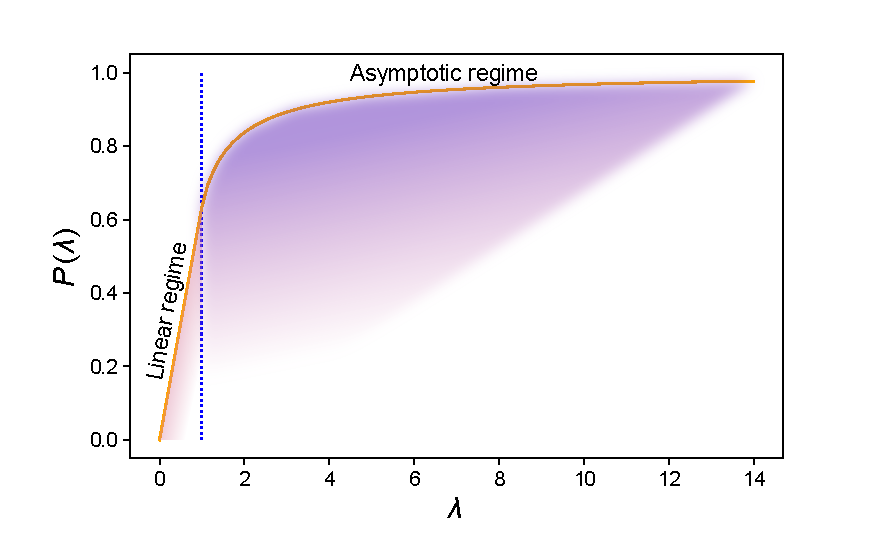
\includegraphics[width=\textwidth]{chapter_fabrication/figures/buffon_probability.pdf}
        \caption[Probability Distribution of a Ribbon Landing Onto a Device]{Probability distribution as a function of the parameter $\lambda$ for a needle tossed onto a grid of equispaced parallel lines. When the needle is short ($\lambda < 1$), the coverage probability increases linearly with the length. When the needle becomes larger than the gap ($\lambda \ge 1$), the probability increases asymptotically to one and is independent of the parameter $\lambda$.}
        \label{fig:fabrication:buffon_probability}
    \end{center}
\end{figure}
%
When $\lambda$ is smaller than zero (Fig.~\ref{fig:fabrication:buffon_probability}), the coverage probability grows linearly with the length of the ribbon. This conclusion can be simply explained by observing that for a fixed grid-spacing distance, using increasingly longer ribbons increases our chances of successfully crossing a graphene nanogap. However, expanding the ribbon length forever is not recommended because the crossing probability drops below one for ribbons much longer than the grid spacing. This results in a device surface covered in ribbons arranged in random directions, with many ribbons covering the same surface area, and increasing the odds of obtaining ribbon adducts and aggregates. This regime may be sufficient for the fabrication of field-effect transistors, but it should be avoided if the goal is to produce single-electron transistors with only one ribbon bridging the nanogap. These straightforward and intuitive ideas have recently been confirmed by \gls{AFM} and electrical transport measurements~\cite{lin2022scaling}.


\section{Deposition Process and Related Phenomena}

One of the key point of a device fabrication are the complex interactions establishing as a consequenche of various surface-related phenomena which occur when an object--in our case, graphene nanoribbons--have to be transferred onto specific substrates \cite{nerngchamnong2013role, huskens2004model}. The rich and wide physics \glspl{GNR} have displayed on substrates where are directly growth remains largely un-matched when ribbons are transferred onto electronic devices; therefore, I argue that a more detailed look at the deposition picture is essential for improving device yield and reproducibility. In order to fulfill this purpose, I qualitatevely studied the effect of different depositon techniques when a solution of liquid-processable nanoribbons was dropcasted on top of the substrate. By substrate here I refer to the a chip where gold and graphene pads have been shaped.

\glspl{GNR} were first diluted in an organic apolar solvent before being drop cast onto the substrate. Apolar solvents have been a valid choice against unwanted charge doping effects of graphene sheets. I have preferably used toluene, choloroform and \gls{THF} to this purpose: this were largely based on the suggestion from our collaborators who synthesised the ribbon I have used and by Dr\. Xuelin Yao. I have also attempted to use higher boiling points solvents such as 1-phenyloctane. The logic behind this choice is that the depositon process is largely dependend on the interactions established between the ribbon and the different surfaces on to of the chip. In order to favour the $\pi-\pi^*$ interactions between the graphene leads and a single graphene nanoribbons strand, a thermodynamic equilibrium between the amount of substance $i$ absorbed on the electrode per unit area, $\Gamma_i$, and the substance in the bulk (the ribbon in the solvent) should be favoured compared to kinetic-related processed such as mass transfer by migration and diffusion.

Given the interactions active between absorbed species the most appropriate adsorption isotherm to use is the Frumkin isotherm, in which the energy of the adsorption process depends on the surface coverage. An estimate of these interactions is provided by first-principle calculations where different anchoring groups such as pyrene and hexabenzocoronene were tested \cite{limburg2018anchor}. The reason to study smaller $\pi$-delocalised systems is related to the smaller computational cost one has to face when simualating such complex interactions at DFT level, and the underlying assumption is that the insights we derive from the simulation are exendible in the case of larger $\pi$-delocalised systems such as \glspl{GNR}.
The interaction between a graphene sheet and a pyrene molecule was estimated to be around \SI{26.3}{\milli\electronvolt}/atom. The large width limit of this value is the binding interaction between two graphene sheets: theoretical estimates pose this value to be between \SIrange{10}{30}{\milli\electronvolt}/atom for a stacking of type $AA$ with an interlayer distance of \SI{3.3}{\angstrom} and about \SIrange{18}{23}{\milli\electronvolt}/atom for a $AB$ stacking with similar graphene-sheet distance \cite{mostaani2015quantum}.

The solvent chlorobenzene (PhCl) was used in this case. As previously stated, the attached alkyl chains significantly improve dispersibility (compared to GNRs without chains). Nonetheless, because GNRs tend to form bundles, they must be sonicated before further processing. The typical sonication parameters were one hour at 50\% power followed by ten minutes at 100\% power 6. The clear, purple colour of a well-sonicated dispersion can be identified (see g. 3.6 (b) inset). If any visible bundles remained, the sonication was repeated for another 30 minutes. Occasionally, a new GNR solution was prepared by diluting a de ned amount of the master solution in 1 ml of PhCl.

It has beeen not possible to perform a more quantitative description through the usage of surface techiniques such as \gls{AFM} or XPS becuase of restrictions put in place due to the Covid-19 pandemic.

\co{Diels-Alder reaction will shift the equilibrium back when heated}

In Ch.~\ref{ch:solubility} and Ch.~\ref{ch:gnrset} Coulomb spectroscopy of liquid-processable GNR will be presented. These GNRs have recently garned attention as the improve
solubility is of paramount importance when ribbons have to be transferred onto a substrate from the solution.

The liquid-phase processability of GNRs is essential for investigating their fundamental physiochemical properties in solution and for the fabrication of nanoelectronic devices via dip coating or drop casting GNR dispersions on solid substrates, and compared with surface-assisted routes, solution-synthesis approaches could be advantageous for large-scale preparation of electronic devices.

In chapters \ref{ch:gnrset} and \ref{ch:solubility}, the Coulomb spectroscopy of liquid-processable \glspl{GNR} will be discussed. The improved solubility these ribbons have demonstrated is of paramount for studying their fundamental physiochemical properties in solution and for fabricating nanoelectronic devices by either dip coating or drop casting on solid substrates~\cite{huang2018supramolecular, narita2014synthesis, niu2019synthetic, yoon2020liquid, saraswat2021materials}.

Several solvents have been qualitatively examined to improve the number of devices with molecular features. The maleimide functionalisation is introduced by using a Diels-Alder reaction to replace the anthracene group along the ribbon edges. This can be written schematically as:

\begin{equation}
    \label{eq:absorption}
    \textrm{MGNR}-\textrm{Anthracene} + \textrm{Maleimide} \xrightleftharpoons[k_{-1}]{k_{+1}} \textrm{MGNR}-\textrm{Maleimide}
\end{equation}


This reaction is reversible, hence it follows the Le Chatelier's principle of equilibrium. When the temperature is increased, the entropic contribution dominates the reaction free energy, which favours the reversal of the equilibrium direction. Even if a faster solvent evaporation is desired after deposition on the device substrate, heating should be avoided. Particularly, the reverse reaction becomes favoured either by heating the solution to close to \SI{100}{\degreeCelsius}, in which case the reaction rate will make the reaction quick, or by maintaining the temperature at approximately \SI{80}{\degreeCelsius} for an extended period of time. As a result, we had to employ solvents with lower boiling points for an optimal deposition. We found THF and toluene to perform significantly better in this regard than 1-phenyloctane or 1,3,5-trichlorobenzene.
